\section{Knowledge-aware Multi-agent Federation}
%\carl{TODO: will work on this section over the weekend}\\
While KGs and LLMs can mutually enhance each other, data are properties and many real-world datasets are privately collected and owned by different institutions, which cannot be simply put together to train more powerful models. 
Moreover, many real-world applications require domain-specific knowledge that may not have been captured by general-purpose KGs and LLMs yet, and such knowledge can also be private properties. 
Finally, while the development of KGs and LLMs is highly automated and data-driven, the values and needs of different human stakeholders may not have been properly reflected in the data and models. 
Federated learning (FL) provides a robust and principled framework for privacy-protected multi-site collaboration, but proper implementation of FL in the new era of generative AI remains unclear; the further incorporation of domain knowledge and human participation is also highly under-explored. In the following, we will envision an innovative Federated Multi-Agent System (FedMAS) for multi-site privacy-protected, knowledge-infused, and human-engaged KG-LLM co-learning scenarios. 


Nowadays, while common practices in AI applications still largely resort to in-house development of models based on public and local data, the successes of generative AI, where complex models are trained with large-scale data, have demonstrated a strong need to collaboratively utilize local data towards obtaining powerful models that can generalize across institutions, finding and utilizing deep data patterns underlying common and rare use cases. Towards protecting local data privacy during collaborative model training, FL provides a promising solution \cite{nguyen2022federated, antunes2022federated, nguyen2022federated, antunes2022federated, xu2021federated, rieke2020future}. However, existing FL frameworks, by merely preventing the direct sharing of training data, are not effective in the scenarios of KG-LLM co-learning, because (1) as the construction of comprehensive KGs necessitates the incorporation of knowledge discovered from local data, private information may get reversely inferred from the collaboratively constructed KG; (2) as powerful generative models like LLMs can easily memorize training data, collaboratively trained LLMs may expose private information facing deliberately composed jailbreaking prompts \cite{wei2024jailbroken, wang2023decodingtrust, xu2024llm}.

In our pioneering studies on FL for graphs \cite{he2021fedgraphnn, xie2021federated, zhang2021subgraph, zhang2024deep, xie2023federated, zhang2022efficient, gu2023dynamic, xie2024federated}, we developed several novel algorithms for different graph separation scenarios. In FedDEP \cite{zhang2024deep}, we developed a prototype-based embedding sharing algorithm with local graph differential privacy (DP) guarantees, and demonstrated its utility in FL for global graph embedding models across private local subgraphs; in FedR \cite{zhang2022efficient}, we showed that sharing relation embeddings across local KGs can help FL for global KG embeddings with less privacy leakage. These studies have laid the foundations for our envisioned framework here, which will build on the private embedding sharing algorithms to construct \textit{multi-view KGs} that can facilitate multi-site knowledge sharing with minimum risks of exposing local private data.

\begin{figure}[htbp]
    \begin{center}
    %\framebox[4.0in]{$\;$}
    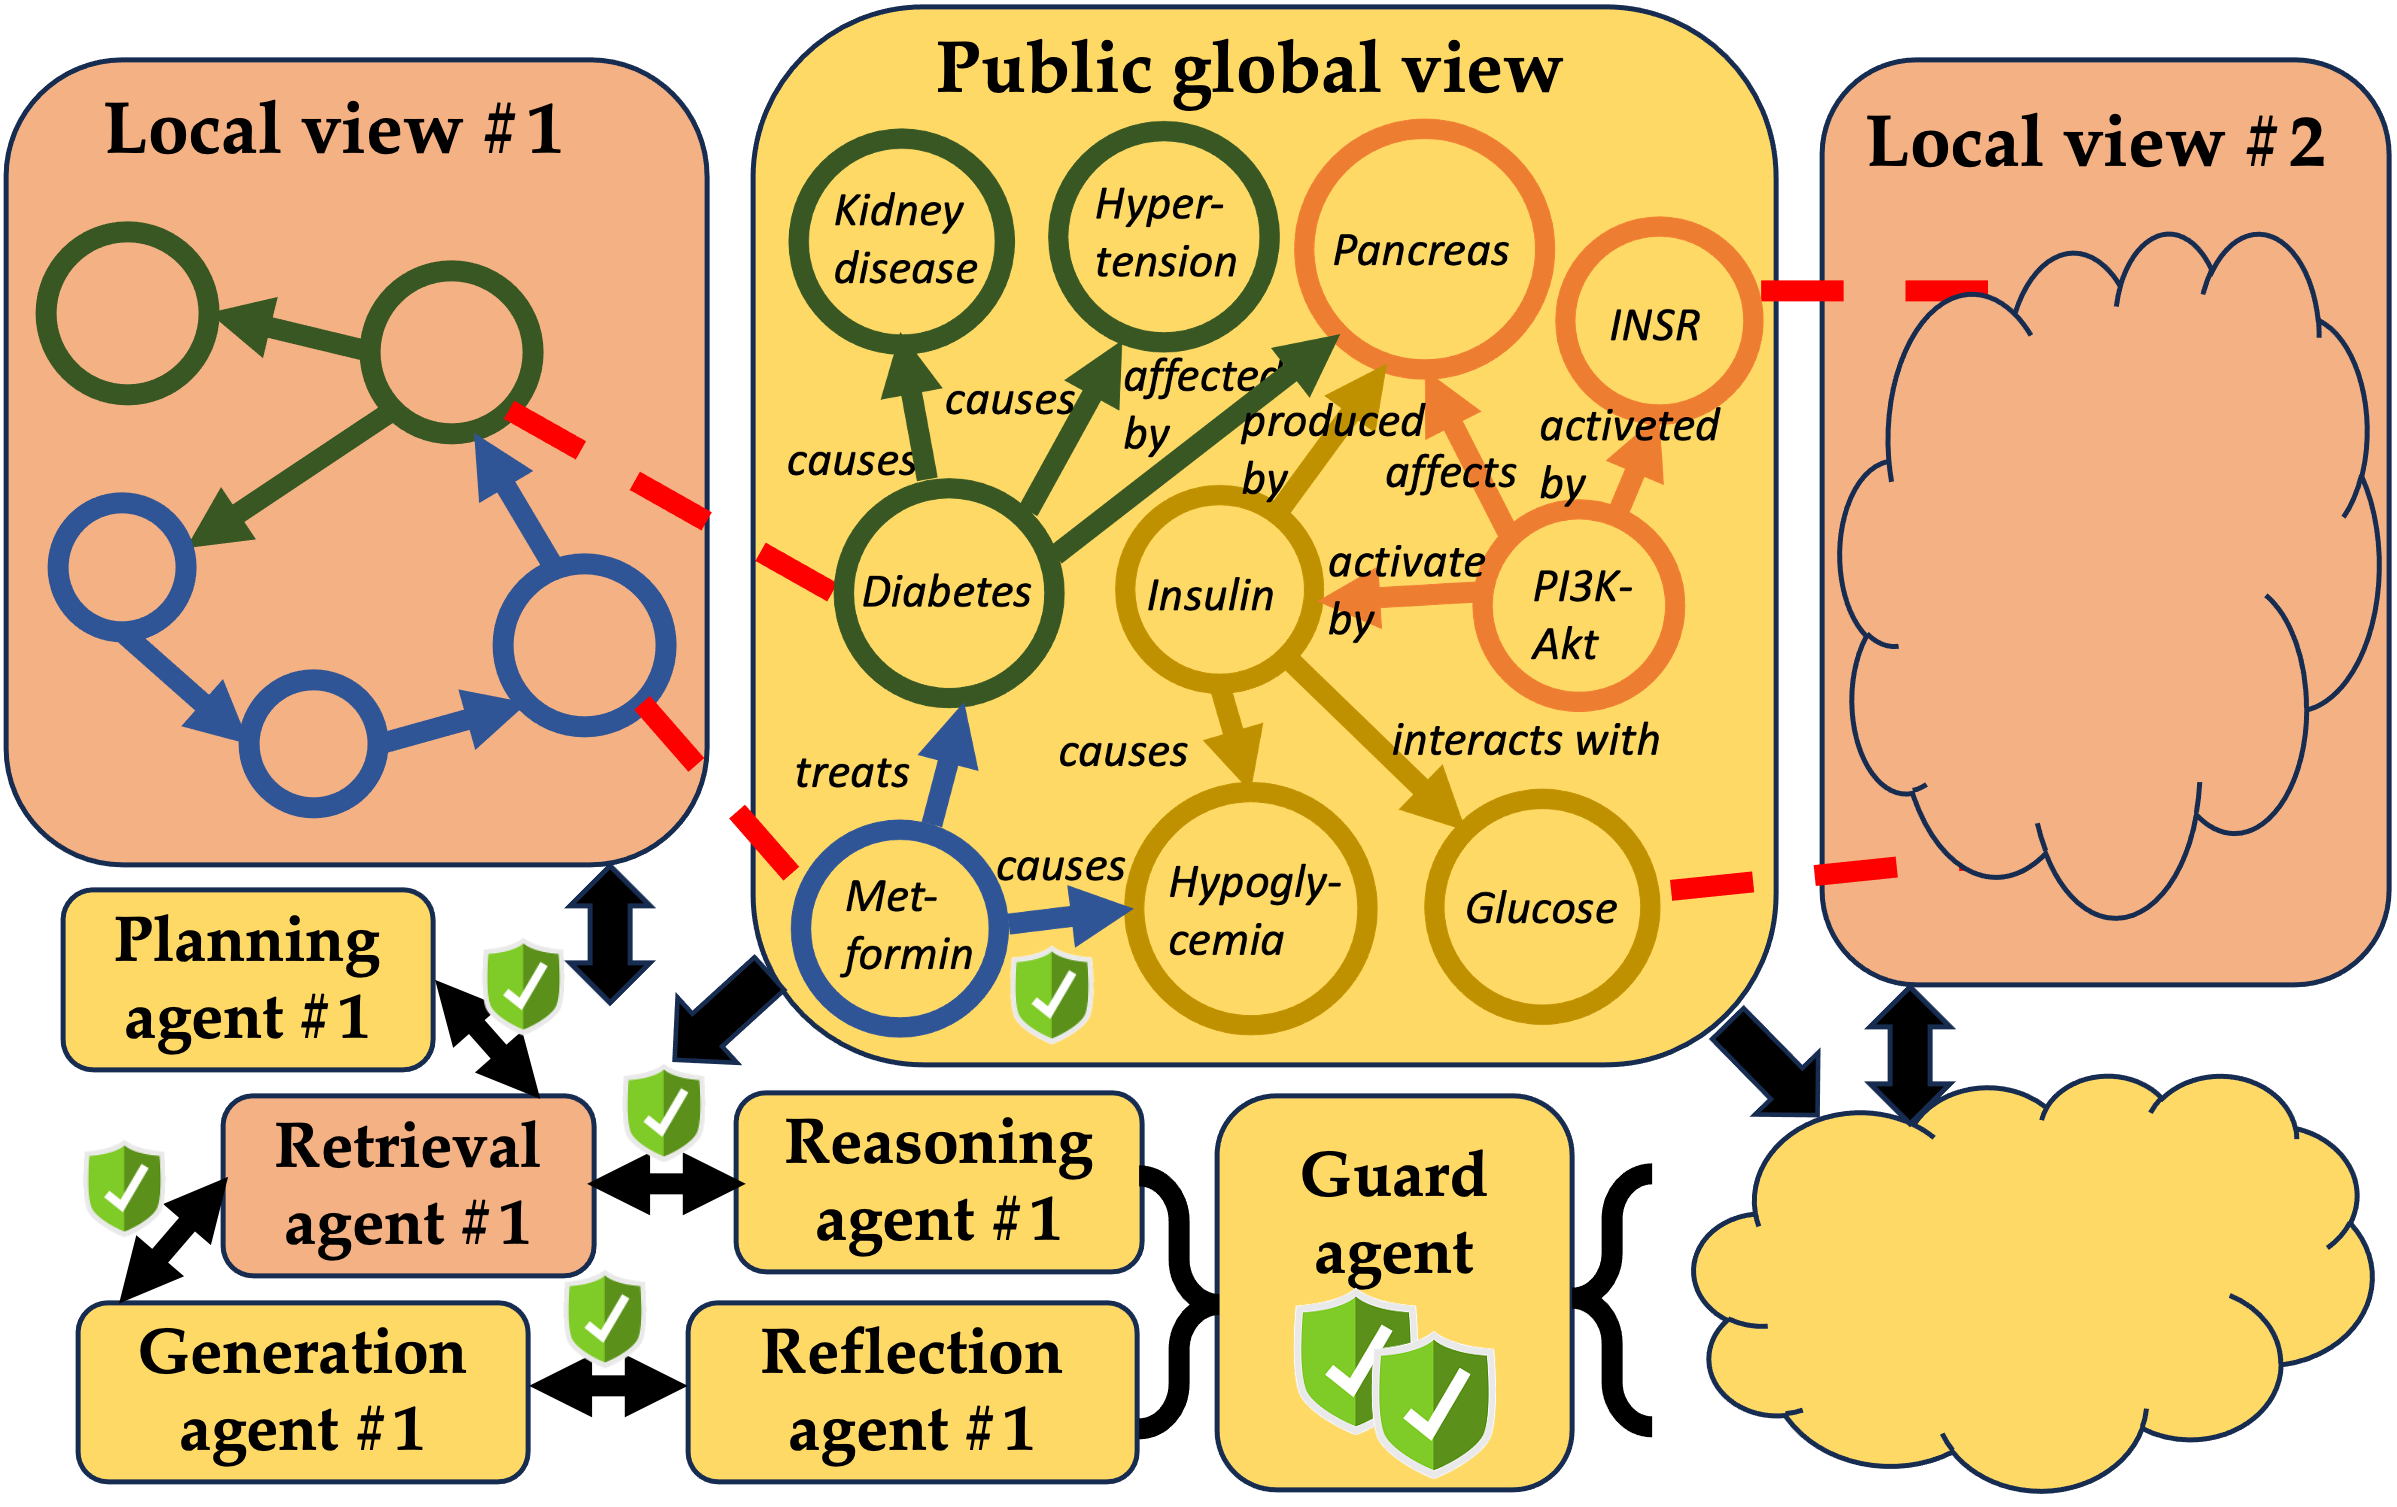
\includegraphics[width=.75\columnwidth]{submissions/CarlYang2024/figures/fedmas.png}
    \end{center}
    % \vspace{-3mm}
    \caption{The envisioned framework of a federated multi-agent system (FedMAS).}
    \label{fig:fedmas}
    % \vspace{-5mm}
\end{figure}

As illustrated in Figure \ref{fig:fedmas}, our envisioned FedMAS will include a multi-view KG and various LLM agents. The federation on KG will be implemented by collectively constructing a multi-view KG by all participating sites, where knowledge from public resources is integrated into the global view, and knowledge from private resources is kept in each site's local view only visible to itself. For each site, entities in its local view are linked with the global view, and only the embeddings related to these linked entities are shared with the server and other sites, via privacy-guaranteed embedding sharing algorithms such as those developed in FedDEP \cite{zhang2024deep} and FedR \cite{zhang2022efficient}. In this way, each local site can compute embeddings on its local view and the public view as if they can see all other sites' local views, allowing them to effectively adjust their local knowledge and further enhance their local LLMs, all without actually seeing the other sites' local views (knowledge). The server will periodically adjust knowledge in the global view also based on the shared privacy-guaranteed embeddings, and apply additional privacy checks to make sure no sensitive knowledge gets propagated into the global view.
%potentially discussing why knowledge is less private and how to avoid inference attack on embeddings

To rigorously protect the more sensitive patient data during the federation on LLM, it is possible to train multiple LLM agents in each site with different functions and let them collaborate through conversations instead of traditional model sharing, so the system can strictly control the level of private data each agent can access and monitor or moderate their collaborations. 
%Based on this design of multi-view KG, we will further enable the federation on LLM by training multiple LLM agents in each site and let them collaborate inside and across sites through conversations. 
%To control the levels of private data access and facilitate the moderation of conversations, each site will train multiple LLM agents focusing on different functions such as planning, retrieval, reasoning, reflection and answer generation. Since all agents will access certain levels of local private data during training and inference, none of them can be directly trained across sites even through FL. To this end, we will build on AutoGen \cite{} to design a structured conversational environment for multi-agent collaboration of LLMs. 
Specifically, since the retrieval agents need to access all local patient data, one plan is to implement programmable guardrails \cite{rebedea2023nemo} on its conversations with all other agents within the same site and forbid them from directly communicating with agents from other sites. Since all other agents can only access patient data indirectly through the retrieval agents, it is possible to adapt techniques such as our recently developed GuardAgent \cite{xiang2024guardagent} based on the clear goals and typical outputs of each agent to monitor all cross-site conversations, detecting and removing any suspicious private information.
%Specifically, since the retrieval and generation agents can directly access local patient data, we will only enable strict one-way conversations from other agents to them; since the planning, reasoning and reflection agents only access local KGs and their performances can likely benefit from cross-site collaborations (such as due to richer knowledge access and more generalized capabilities), we will enable two-way conversations among them cross sites; when the system is normal, we do not expect the agents to ask or answer privacy sensitive questions, and since each agent has clear goals, it will also be relatively easy to detect abnormal conversations; we will also explore techniques such as DP-prompting \cite{} to moderate the conversations against privacy leakage, and conduct red teaming \cite{} to rigorously monitor the conversations.  

When applying FedMAS to specific application domains such as finance, law, education, and healthcare, it is promising to leverage the knowledge-based data sharing mechanism to incorporate existing domain knowledge towards further alleviating knowledge gaps and mitigating potential biases. 
Built on recent promising results from LLM-based data annotations as discussed in Section 2, FedMAS can utilize specialized LLM agents to perform comprehensive extraction of structured knowledge from existing guidelines and tutorials and automatically integrate them with existing general and domain-specific KGs. For example, in healthcare, one type of important domain-specific entity is social determinants of health (SDOH) \cite{artiga2020disparities, artiga2018beyond, who2008closing}. The system can start with a set of known SDOH such as defined by WHO \cite{marmot2005social, phelan2010social}, and further extend the set and discover their impacts and relationships with various risk factors by investigating relevant healthcare literature. The KGs enhanced through these steps are supposed to facilitate the alleviation of various health disparities when utilized by subsequent LLM agents in the FedMAS. 
%Specifically, we will (1) adapt techniques in Thrust 1 with a focus on identifying SDOH-related entities and relations, such as by using the key factors in Figure \ref{fig:t3-3} to create an initial SDOH ontology and using LLMs for its further expansion to include more fine-grained factors; (2) conduct controlled experiments by finding and synthesizing pairs of patient data which only differ by certain SDOH factors, and analyzing LLM outputs for them regarding different clinical questions; (3) based on insights from (2), design programmable guardrails \cite{rebedea2023nemo} to enforce LLMs to output SDOH-removed predictions for tasks such as disease diagnosis where fairness is concerned, and output SDOH-informed predictions for tasks such as treatment suggestion where patients' financial abilities and access to healthcare resources should be considered.

While FedMAS utilizes AI advances to automate multi-site data integration and modeling, comprehensive and trustworthy AI systems need to also incorporate the values and needs of various stakeholders, who can have different and even contradictory perspectives. LLMs, especially in our multi-agent conversational environment, provide unique convenience for effective and efficient human participation, where different stakeholders can verify, influence, and complement the decision processes and outputs of different LLM agents, all based on natural languages as the interface.
Specifically, we envision a novel multi-stage intervention mechanism to efficiently enable the participation of different stakeholders in the LLM-based multi-agent conversational environment. The potential stages could include (1) LLM uncertainty quantification, where LLMs highlight their own uncertain outputs; (2) Rubrics-based rating, where humans create rubrics to automatically rate the LLM outputs; (3) Focused human interactions, where humans directly interact with LLMs, focusing on the problematic scenarios identified in the previous stages. The overall multi-stage mechanism is supposed to allow FedMAS to adapt to human values through iteratively integrating the language-based feedback via interactions with various stakeholders. 

%Instead of having the stakeholders freely chat with LLM agents, the mechanism will work as follows: Stage-1 (Uncertainty): LLM uncertainty quantification methods \cite{farquhar2024detecting, lu2024uncertainty} will be performed to identify potentially problematic answers such as due to hallucinations or data biases; Stage-2 (Rubrics): Rubrics manually generated from stakeholder feedback on a small development set such as based on the guidelines in Figure \ref{fig:t3-2} will be applied to automatically rate new LLM outputs, further exploring or highlighting problematic answers. Stage-3 (Human): Limited and costly human interactions will focus on problematic LLM outputs detected through the previous stages; %, either (partially) following the feedback guidelines or through free-form conversations; the stakeholders will also participate in elaborated surveys after interactions with LLMs, to summarize thoughts and concerns. On a development set, we will have the three stages cross-validate each other to evaluate their individual effectiveness and uncover potentially missed problematic LLM outputs in each individual stage. The uncertainty measurements, rubrics and feedback guidelines will be revised iteratively after the stakeholder surveys and cross-stage validations.
